\documentclass[a4paper]{scrartcl}
\usepackage{bogwonch}
\newcommand{\new}[1]{{\color{BrickRed}#1}}

\title{Authorization Logic for Mobile Ecosystems}
\subtitle{Third Year Report}
\author{Joseph Hallett}
\date\today

\begin{document}
\maketitle

\begin{abstract}
  This report describes the progress made in the third year of my PhD. It
  describes my work this year on BYOD policies and encoding them in AppPAL, a
  policy language for the Android mobile ecosystem, as well as work developing
  AppPAL policy analysis tools and a probabilistic variant of AppPAL, as well as
  plans for how this should continue in the time remaining. The report goes on to
  describe my plans for the thesis and gives a table of content as well as a plan
  for submission by June 2017.
\end{abstract}

\section{Introduction}
\label{sec:introduction}

Users can choose from a large range of apps for their phones. Their devices have
access to a huge amount of personal information, and despite improvements giving
users more control over what information they share, users still have to be
careful to ensure their privacy and data-security preferences are followed.
These devices are increasingly entering every part of their user's lives being
used for work as well as for home.

The interactions between people and mobile devices requires an increasing number
of trust relationships and policies---rules that describe how a device or user
should behave. These trust relationships take the form of delegations of
responsibilities to third parties, for example a user might delegate to a store
to check that their apps are not malicious.


These policies and trust relationships are often ad-hoc and informally
specified. Users are not clear about how they want their apps to behave.
Businesses specify policies for users' devices in their workplace using natural
language. Different app marketplaces have different policies describing how
their users and developers can use their store and what rights they have, but
these are hidden behind long EULAs and developer agreements. The interactions
between users, their devices, their employers, the stores they buy apps from and
the apps themselves forms a vibrant mobile ecosystem of requirements,
preferences and trust relationships for users who are often left to understand
and enforce these relationships on their own.

Authorization logics are designed to express policies precisely, and make
decisions on the basis of facts. They have been used to implement access control
systems (deciding whether someone has access to a file or not).  By using these
formal systems we can make informal policies in the mobile ecosystem
more precise, we can start to automate enforcement and make comparisons between
the different entities in the ecosystem on the basis of their roles and
responsibilities.

\subsection{Goals of this PhD}

The goal of this work is to create a practical scheme for linking the high-level
human policies in the mobile ecosystems, to the technical means for enforcing
policies.
The work will focus on the ecosystems surround Google's Android operating system, the
largest mobile OS.  Unlike iOS (the OS for Apple's devices), there is a greater
variation in the app stores available (Play Store, Amazon App Store, Yandex,
Baidu and Qihoo 360 to name but a few) as well as a broader amount of research
on Android's apps and permission systems.
% TODO: citations please


Much prior work has focused on the
technical side of policies; extending Android with more sophisticated permission
systems and complex enforcement schemes.  This work differs in that it focuses
on the human policies, and is happy to delegate the precise enforcement
mechanism to a tool.

To do this I have taken an existing authorization language, SecPAL, and applied
it to the problem of formalising the user level policies in mobile ecosystems
(and in doing created a modified implementation of SecPAL called \emph{AppPAL})
Specifically I aim to show:

\begin{itemize}
\item That authorization languages with named speakers (specifically AppPAL) are
  a good fit for describing the policies and trust relationships surrounding
  Android.
\item That users have policies but that they struggle with enforcing them in
  practice.
\item That AppPAL can be used to build systems where policies can be
  enforced by delegation to tools, and the details of implementing such a system.
\item To show how AppPAL can be used to describe precisely the differences
  between different policies (be they BYOD policies in companies, developer
  agreements in stores or app preferences), and identify problems
  with them ahead of time.
\end{itemize}


% TODO: What is the ``thesis of the thesis''? (a stupid DA term).
% It is basically the goals but refutable.

\section{Progress}
\label{sec:work}

Last year, I worked on implementing AppPAL on Android, built a security
knowledge base to store results from static analysis checkers and metadata about
apps. I surveyed user and developer policies present in stores and
their distribution mechanisms. I also investigated whether users install apps
matching their privacy preferences and presented a draft of a paper, that was
later accepted and published~\cite{hallett_apppal_2016} and is included in the appendix.

This year I proposed working on a case-study looking at BYOD policies and
developing a knowledge distribution protocol to define how AppPAL assertions
should be distributed.  Work on the BYOD policies has resulted in a presentation
at iFM's doctoral symposium~\cite{hallett_specifying_2016}, but there hasn't
been progress working on a knowledge distribution protocol.  Instead, I have been
worked on developing analysis tools for AppPAL policies and started creating a
probabilistic variant of AppPAL.

\subsection{Typed AppPAL}
\label{sec:types}

\begin{lstlisting}[language=Python, float, caption={Procedure used to expand types from AppPAL into SecPAL.}]
def expand_types(a: Assertion) -> Assertion:
  for v in a.head.vars():
    if v.type != None:
      f = Fact(v, 'is'++str(v.type))
      a.body.add(f)
  return a
\end{lstlisting}

SecPAL's safety condition requires all variables in an assertion's head to be
used in the body. When trying to describe policies a common pattern is to say a
variable in an assertion belongs to a certain domain. For example someone who
satisfies some property (for example they are a staff member) can make
statements about apps.
For example, Alice might be willing to let her friends say what apps are
suitable for her children.  This could be expressed in SecPAL as follows:

\begin{lstlisting}
'alice' says Friend can-say App isSuitableFor(Child)
  if Friend isFriend, App isApp, Child isChild.
\end{lstlisting}

The conditionals in this assertion add unnecessary noise to the assertion. We
know from the names of the variable what set of constants might be used
to instantiate it (Alice's \emph{friends}, \emph{apps} or \emph{children}). To
avoid this noise I added a sugared syntax to AppPAL that allows variables to
declare their \emph{type}. Using the sugared notation the above statement
becomes:

\begin{lstlisting}
'alice' says Friend:F can-say App:A isSuitableFor(Child:C).
\end{lstlisting}

\begin{figure}
  \newcommand{\nonterminal}[1]{$\langle$#1$\rangle$}
  \newcommand{\terminal}[1]{\textbf{#1}}
  \begin{tabular}{r c l}
    \footnotesize
    \nonterminal{E}         & $\coloneqq$ & \nonterminal{Variable} $\vert$ \terminal{'constant'} \\
    \nonterminal{Variable}  & $\coloneqq$ & \new{(\terminal{Type}\terminal{:})?}\terminal{VariableName}
  \end{tabular}
  \caption{Changes to SecPAL's variable syntax.  Additions are shown in \new{red}.}
  \label{fig:apppal-types}
\end{figure}
The changes to SecPAL's syntax is shown is \autoref{fig:apppal-types}.
After an assertion has been parsed the variables with types are extracted for
each variable a conditional is added that \texttt{VariableName \emph{is}Type},
and the types are removed from the variables.

This gives a cleaner policy language however it also means that the predicates
used start to have some intrinsic meaning.  A predicate starting with
\texttt{is} describes some property of the predicate's subject.
SecPAL did not require predicates follow any naming conventions, however with
AppPAL we have started to give predicates meaning based on their name.
This is expanded in the \autoref{sec:byod} where we describe other predicate
prefixes that we use for specific purposes.

\subsection{BYOD Policies}
\label{sec:byod}

Employees increasingly bring their own devices to work. Around 70\% of all
companies having some form of \ac{BYOD} scheme~\cite{schulze_byod_2016}. In
hospitals the use of personal devices as part of patient care is even more
common. One survey from the UK found that around 80\% of surgical doctors were
willing to use their personal devices for work, with 85\% regularly using them
to look up information, and 50\% having medical apps already installed on their
phones~\cite{patel_uk_2015}. Another survey from the US found similar numbers of
physicians regularly using their devices as part of their
work~\cite{moyer_managing_2013}.

Whilst there has been plenty of work looking at how to enforce BYOD policies,
there has been something of a push-back against automatically enforcing them.
Whilst \ac{MDM} software can enforce some policies by blacklisting or rewriting
apps to use guarded APIs having an \ac{MDM} package does not guarantee a
company's BYOD policy is enforced correctly, or even enforced at all.  One survey of
companies using \ac{MDM} software found that over half of them had devices that
broke their policies within their
networks~\cite{mobileiron_security_labs_q4_2015}.
Whilst the majority of BYOD policies are relatively simple: a report from the
healthcare sector, where policies are typically more complex, noted that:

\begin{quote}
  ``an approach toward educating the users instead of trying to control the
  technology may be more practical in the short term.''~\cite{moyer_managing_2013}
\end{quote}

The tension between \ac{MDM} software and having something that employees can
understand has possibly led to many BYOD policies being published using natural
language. Whilst there has been much research on the \emph{technical} means to
enforce BYOD
policies~\cite{martinelli_enhancing_2016,armando_enabling_2014,costantino_towards_2013}
there has been little work comparing the natural languages of the policies in an
effort to find the common idioms and requirements the companies want to enforce,
as well as making precise comparisons between policies.

I have taken policies from five different sources as part of a case study into
the rules and idioms used in BYOD policies.  One is from the SANS
institute and serves as a guide for companies seeking to implement their own
BYOD policy, one is from HiMMS and is a guide for hospitals looking to implement
a BYOD policy.  Another from an NHS trust is a complex policy describing
how medical staff should use their own devices when dealing with patients, as
well as BYOD concerns.  The other two are simple BYOD polices typical of what
most companies implement and are taken from Edinburgh University and a company
selling emergency sirens.

I have used AppPAL to create a formalisation of each of the policies. This has
helped identify common predicates used in each of the policies
(\autoref{tab:byod-predicates}). It has also led to a set of
standard prefixes for AppPAL predicates. In \autoref{sec:types}, I described how
predicates that start with \emph{is} are reserved for predicates that give a
type to their subject. Through translating the BYOD policies I found four
distinct categories of predicate that could encode all the different rules in
each of the policies as well as many similarities in concerns for BYOD
policies.


\begin{table}\centering\footnotesize
  \newcommand{\angledtitle}[1]{\rlap{\rotatebox{30}{#1}}}
  \sffamily
  \begin{tabular}{l c c c c c p{0.45\linewidth} }
    % \toprule
    Predicate                                   & \angledtitle{Code3PSE} & \angledtitle{Edinburgh} & \angledtitle{HiMMS} & \angledtitle{NHS} & \angledtitle{SANS} & Description                                                                          \\
    \midrule
    Device \texttt{canBackupTo}(Server)         &                        & \cmark                  & \cmark              &                   &                    & Says the device may send backups to a server.                                        \\
    Device \texttt{canCall}(Number)             &                        &                         &                     & \cmark            & \cmark             & Says the telephone numbers a device can call.                                        \\
    Device \texttt{canConnectToAP}(AP)          &                        &                         & \cmark              &                   & \cmark             & Says a device may associate with an access point.                                    \\
    Device \texttt{canConnectToNetwork}(Subnet) & \cmark                 &                         &                     &                   & \cmark             & Says the device may connect to a network, for example computers all within a subnet. \\
    Device \texttt{canConnectToServer}(IP)      &                        &                         &                     & \cmark            & \cmark             & Says the subject (a device) can connect to a given server (identitfied by a URL).    \\
    Device \texttt{canInstall}(App)             &                        &                         &                     & \cmark            & \cmark             & Says the device may install an app.                                                  \\
    User \texttt{canMonitor}(Device)            & \cmark                 &                         &                     & \cmark            & \cmark             & Says the subject (a user) can monitor and unlock a device.                           \\
    Device \texttt{canStore}(File)              &                        &                         & \cmark              &                   & \cmark             & Says a device may store some data in permanent (non-transient) storage.              \\
    User \texttt{canUse}(Device)                &                        &                         &                     & \cmark            & \cmark             & Says a user may use a device.                                                        \\
    User \texttt{hasAcknowledged}(Policy)       & \cmark                 & \cmark                  & \cmark              & \cmark            & \cmark             & Says an individual has acknoweldged a policy.                                        \\
    Device \texttt{hasFeature}(Feature)         &                        & \cmark                  &                     & \cmark            &                    & Says a device has a feature enabled.                                                 \\
    Something \texttt{hasMet}(Policy)           &                        & \cmark                  &                     & \cmark            & \cmark             & Says a something has met a given set of requirements.                                \\
    Device \texttt{isActivated}                 &                        &                         & \cmark              & \cmark            & \cmark             & Specifies a device has been activated for BYOD usage.                                \\
    App \texttt{isApp}                          & \cmark                 &                         & \cmark              & \cmark            & \cmark             & Specifies an app.                                                                    \\
    Something \texttt{isApproved}               &                        &                         & \cmark              &                   & \cmark             & Specifies that something has been vetted and approved of.                            \\
    Data \texttt{isData}                        & \cmark                 &                         &                     &                   & \cmark             & Specifies data.                                                                      \\
    Device \texttt{isDevice}                    & \cmark                 & \cmark                  & \cmark              & \cmark            & \cmark             & Specifies a device.                                                                  \\
    User \texttt{isEmployee}                    & \cmark                 & \cmark                  &                     & \cmark            & \cmark             & Specifies that someone is an employee.                                               \\
    Device \texttt{isEncrypted}                 &                        & \cmark                  &                     & \cmark            & \cmark             & Specifies a device is encrypted.                                                     \\
    Feature \texttt{isFeature}                  & \cmark                 &                         &                     &                   & \cmark             & Specifies a feature.                                                                 \\
    App \texttt{isInstallable}                  &                        &                         &                     & \cmark            & \cmark             & Specifies an app is installable.                                                     \\
    Device \texttt{isLost}                      & \cmark                 &                         & \cmark              & \cmark            & \cmark             & Specifies a device is missing.                                                       \\
    Device \texttt{isOwnedBy}(User)             & \cmark                 & \cmark                  & \cmark              & \cmark            & \cmark             & Specifies something's owner.                                                         \\
    File \texttt{isSecurityLevel}(Level)        &                        &                         & \cmark              &                   & \cmark             & Specifies some data as having business sensitive information.                        \\
    Something \texttt{isString}                 & \cmark                 &                         &                     & \cmark            &                    & Specifies a string.                                                                  \\
    Number \texttt{isTelephoneNumber}           &                        &                         &                     & \cmark            & \cmark             & Specifies a telephone number.                                                        \\
    Device \texttt{mustDisable}(Feature)        & \cmark                 & \cmark                  &                     & \cmark            & \cmark             & Forces the disablement of a feature (or a device).                                   \\
    User \texttt{mustInform}(User, Something)   & \cmark                 &                         & \cmark              & \cmark            & \cmark             & Forces someone to disclose something to someone.                                     \\
    Device \texttt{mustWipe}                    & \cmark                 &                         & \cmark              & \cmark            &                    & Forces a device to be erased.                                                        \\
    \bottomrule
  \end{tabular}
  \caption{Summary of predicates used in multiple BYOD policies.}
  \label{tab:byod-predicates}
\end{table}

\begin{table}
  \centering\footnotesize
  \newcommand{\pform}[3]{\textit{#1}~\textbf{#2}#3}
  \begin{tabular}{l p{0.5\linewidth}}
    \toprule
    Prefix                            & Meaning                                                                     \\
    \midrule
    \pform{subject}{can}{Action}      & The subject is allowed to perform the action.                               \\
    \pform{subject}{has}{Action}      & The subject has performed the action.                                       \\
    \pform{subject}{is}{Property}     & The property holds true for the subject.  Mostly used for typing statments. \\
    \pform{subject}{must}{Obligation} & The subject is required to satisfy the obligation                           \\
    \bottomrule
  \end{tabular}
  \caption{Standard prefixes for AppPAL predicates}
  \label{tab:predicate-conventions}
\end{table}

\subsubsection*{Future Directions}

I have gone as far as translating the policies, and ensuring they use
semi-standard terms and AppPAL predicates,  and have also developed some
rudimental tools for visualising the policies and what responsibilities each
speaker has.  I plan to make comparisons between each of the policies and
describe a standard set of predicates and tooling for reasoning about BYOD
policies.

This  work should ideally lead to a publication, perhaps at
iFM\footnote{Based on last year's CFP the submission date would be early January.} where
earlier work on this was presented in their doctoral
symposium~\cite{hallett_specifying_2016}.

All the BYOD policies I have looked at make use of acknowledgments by the
subjects of the policy that they will follow, or be aware of, certain rules.
These are interesting as they cannot be enforced by tooling (which looks at
technical means to prevent devices from performing actions).  These
acknowledgments may carry certain legal responsibilities; it would be
interesting to look at how these can be collected, what delegations of trust
are made within them, and what responsibilities each speaker has.  Working out
what responsibilities a speaker has and what delegations are made is, of
course, recoverable from the trace of a dynamically evaluated AppPAL policy.
It would be nice however to do this statically.

I had hoped to develop some analysis tools that might spot problems with the
policies automatically (described~in~\autoref{sec:lint}) but the current state
of BYOD policies is that most are too simple to have problems, and the faults in
longer policies are limited to rules being duplicated or underspecified
rather than more interesting problems,  such as having multiple ways of
satisfying a rule which can undermine the security goals.

\subsection{Automatic Analysis of Policies}
\label{sec:lint}

When examining an AppPAL policy it is natural to wonder whether the policy is
as optimal (in terms of the rules and facts required to decide a query, with
respect to the number of rules in the policy) as it could be, or whether a
decision is even reachable given the rules and facts contained in the policy.
Does an assertion context (i.e.~the assumptions available to prove a statement) contain enough statements to use a given rule? If
there are multiple ways of deciding whether some statement is true or not does
one rule require fewer statements than any other? Does one rule require only a
subset of the facts of another rule, implying the second is redundant?

\subsubsection{Checking Satisfiability}

Inference in AppPAL happens by collecting ground facts and constraints that
satisfy rules. These rules are combined to form a policy. When a rule is
satisfiable there is a combination of facts that could satisfy
its conditionals. If there are no facts that could satisfy the rule then the policy may be incomplete as there are rules that can never be
used.  Formally for any goal $G$:
\begin{align*}
  G \in \text{Satisfiable}~\text{\textit{if}}~\exists A \in \text{AC}:~&\exists \theta:~G\equiv\text{head}(A\theta) \\
                                                              \wedge~ & (\text{conditionals}(A) = \emptyset \\
                                                                      & \vee~\forall G^\prime \in \text{conditionals}(A).~G^\prime \in \text{Satisfiable}.)
\end{align*}

This is a similar idea to the notions of \emph{satisfiability} in Datalog (and
more generally logic programming).  Satisfiability in Datalog is defined
as~\cite{alon_levy_equivalence_1993}:

\begin{quote}
  \textbf{Satisfiability:} An IDB predicate $s$ of a program $P$ is
  \emph{satisfiable} if there is some EDB $D$, such that $P$ defines a
  non-empty relationship for $s$.
\end{quote}

SecPAL does not necessarily\footnote{It is implementation dependant. If a
  translation to Datalog$^C$ was used as suggested by
  Becker~\cite{becker_secpal:_2010} then it might.} splits it's assertion
  context into an EDB (extinsional database, essentially the ground facts) and
  IDB (intensional database, relations defined by rules).  If a Datalog
  predicate is taken as a SecPAL goal, a Datalog program is taken as a number
  of SecPAL assertions, and the EDB is taken as AppPAL ground facts (i.e.
  assertions with no conditionals) then the definition is equivalent.

For example of satisfiability, consider the following snippet taken from the
NHS policy described in \autoref{sec:byod}.  The rule described in the policy
is that an app must be approved by the \emph{integrated governance commitee} as
well as by either the \emph{care and clinical policies group} as well as the
\emph{management of information group} depending on whether it is for clinical
or business use. We can describe this in AppPAL as follows:

\begin{lstlisting}
'nhs-trust' says App isInstallable
  if App isApproved, App isUsableClinically.
'nhs-trust' says App isInstallable
  if App isApproved, App isUsableNonClinically.
'nhs-trust' says 'igc' can-say App:isApproved.
'nhs-trust' says 'cacpg' can-say App:A isUsableClinically.
'nhs-trust' says 'mig' can-say App:A isUsableNonClinically.
\end{lstlisting}

This is all very well, but what apps in practice are approved for use.
As the policy document notes, none of the groups or committees have ever
approved an app in practice.  When we run the satisfiability checker on this policy
it reports that (amongst other information) no app is installable.

\begin{lstlisting}
$\$$ java -jar Lint.jar --satisfiability example.policy
[I]: loaded 1/1 files of 6 assertions
Issues identified when checking satisfiability.
The following decisions may be unsatisfiable by their speakers:
'nhs-trust' says * isUsableClinically
'nhs-trust' says * isInstallable
'nhs-trust' says * isApproved
'nhs-trust' says * isUsableNonClinically

In particular the following assertions are unsatisfiable:
'nhs-trust' says App isInstallable if App isApproved, App isUsableNonClinically.
'nhs-trust' says App isInstallable if App isApproved, App isUsableClinically.

These decisions may be satisfiable through delegation but we
lack any statements to that effect from the delegated party:
(via 'cacpg') 'nhs-trust' says * isUsableClinically
(via 'igc') 'nhs-trust' says * isApproved
(via 'mig') 'nhs-trust' says * isUsableNonClinically
\end{lstlisting}

As well as reporting which decisions it cannot make, it also reports the
specific assertions as well as which decisions could be reached, but rely on
delegation, and we have no information from the delegated speakers.  This could
be because the delegated parties do not believe any app is approved, or it could
be because we haven't asked them yet and imported their statements.

This check is somewhat simple and we don't take into account dependencies
between variables.  If we add, for example, the statements:

\begin{lstlisting}
'igc' says 'angry-birds' isApproved.
'cacpg' says 'dropbox' isUsableClinically.
'mig' says 'instagram' isUsableNonClinically.
\end{lstlisting}

Then we will still never find any installable apps, as the IGC, CACPG and MIG
need to agree on the same app to find it installable.  When we run the
satisfiability checker however, we find no problems as all the decisions are now
satisfiable as there is a decision about \emph{some} variable; even if that
variable isn't useful in practice.

\begin{lstlisting}
$\$$ java -jar Lint.jar --satisfiability example.policy
[I]: loaded 1/1 files of 11 assertions
[I]: no completeness problems
\end{lstlisting}

The satisfiability checker acts as a quick sanity checker that a policy contains
enough facts and rules to use all of the rules in the policy; unlike AppPAL
proper which can check any specific decision.

%The code in \autoref{alg:reachable} produces a set of pairs of predicates and
%speakers where the pair of a speaker and a predicate indicates that that
%speaker may say something about that predicate. We search over all the
%assertions in the AppPAL assertion context. If all of an assertion's
%conditionals (the facts in the if part) are reachable (or it has none) then the
%speaker and predicate are added to the reachable set. If the statement is a
%can-say statement then we additionally check if the delegated predicate is
%reachable from the delegated speaker, and if so mark the delegated statement as
%reachable from the speaker who made the can-say statement.
%
%\begin{lstlisting}[language=Python,float,caption={Procedure for finding all reachable assertions.},label={alg:reachable}]
%def reachable(ac) -> set:
%  reachable = new set()
%  iterate = True
%  while iterate == True:
%    iterate = False
%    for assertion in ac:
%      e = a.speaker
%      p = a.predicate
%      if p.isCanSay() and (e, p) in reachable:
%        if (p.delegator, p.delegation) in reachable:
%          if for all c in a.conditions: (e, c.predicate) in reachable:
%            reachable.add((e, p.delegation))
%            iterate = True
%      else if not (e, p) in reachable:
%        if for all c in a.conditions; (e, c.predicate) in reachable:
%          reachable.add((e, p))
%          iterate = True
%  return reachable
%\end{lstlisting}

\subsubsection{Checking Redundancy}

In logic programming there are two types of redundancy~\cite{alon_levy_constraints_1992}:
\begin{itemize}
\item \emph{Unreachability} occurs if a predicate does not take part in the
  minimal deverivation tree of a fact.
\item \emph{Irrelevance} occurs if a derivation tree contains pairs of identical atoms.
\end{itemize}

% TODO: sort this crap out.  make sure I'm using the terms from logic programming/

Redundancy occurs when there are multiple rules that result in the same decision being
made.  Rules may depend on other rules, or ground facts.  One proof ($A$) is made
redundant by another proof ($B$) if the set of ground facts used in $B$ is a
subset of the ground facts used in $A$. Whenever $A$ is satisfied $B$ will also
be, but when $B$ is satisfied $A$ may not be: consequently $A$ is redundant as
$B$ can be used to prove its goal with fewer facts.
Formally for any goal $G$.
\begin{align*}
  \exists p_1 \in \text{proofs}(G).~\exists p_2 \in \text{proofs}(G).        & \\
  p_1 \not= p_2~\wedge~\text{facts}(p_1) \subset \text{facts}(p_2)           & \implies G\text{ has redundant proofs.} \\
  p_1 \not= p_2~\wedge~\text{facts}(p_1) = \text{facts}(p_2)                 & \implies G\text{ has equivalent proofs.}
\end{align*}
Additionally if two different goals ($G$ and $G^\prime$) have equivalent proofs, then we report this
as it implies the two statements may not be independent.
\begin{align*}
  \exists p_1 \in \text{proofs}(G).~\exists p_2 \in \text{proofs}(G^\prime). & \\
  \text{facts}(p_1) = \text{facts}(p_2)                                      & \implies \text{$G$ and $G^\prime$ have equivalent proofs.}
\end{align*}


A simple example might be the policy shown in \autoref{fig:redundancy-graph-simple}.
The second rule makes the first redundant.  We can represent the policy
as a graph shown opposite the policy.  The goal (shown as a blue rectangle) has two routes
to prove it true (each shown in ellipses).  Route 1 requires that the facts
(shown in green rectangles) \lstinline!'x' says 'y' r,! and
\lstinline!'x' says 'y' q.!, whereas route 0 only requires the
latter fact.

\begin{figure}
  \centering
  \begin{minipage}{0.4\linewidth}
    \begin{lstlisting}
'x' says 'y' p
  if 'y' q,
     'y' r.

'x' says 'y' p
  if 'y' q.
    \end{lstlisting}
  \end{minipage}
  \begin{minipage}{0.59\linewidth}
    \scriptsize{}
    \def\svgwidth{\columnwidth}
    \import{figures/}{redundancy-simple.pdf_tex}
  \end{minipage}
  \caption{A simple policy shown as a graph.}
  \label{fig:redundancy-graph-simple}
\end{figure}

A more complex example is shown bellow:
\begin{lstlisting}
'x' says 'z' p if 'z' q.
'x' says 'y' can-say 'z' p.
'y' says 'z' p if 'z' q.
'y' says 'x' can-say 'z' q.
\end{lstlisting}
Representing this policy as a graph we find it is more complex. Goals that
depend on more than just green facts, are shown as black rectangles.  If a goal
is used to prove another goal, and it itself only depends on green, ground,
facts, then the node is marked to be flattened (red rectangle).  Its proofs are
merged into the higher proof, and the flattened goal is removed from the higher
proof.  This process is repeated until no more nodes can be flattened (shown
twice in \autoref{fig:redundancy-complex}).  Once the graph is flattened we can
identify that \lstinline!'x' says 'z' p! has a redundant means of proof (route
0 only uses one of route 1's facts).  We can also see that all the proofs for
\lstinline!'y' says 'z' q! and \lstinline!'y' says 'z' p! use the same facts.
We report these statements as having equivalent proofs as the goals are not
independent of each other (implying we could use fewer goals and still write
equivalent policies).
\begin{figure}
  \centering\tiny
  \framebox{\def\svgwidth{0.35\textwidth}1.
    \import{figures/}{redundancy-complex-0.pdf_tex}}
  \framebox{\def\svgwidth{0.55\textwidth}2.
    \import{figures/}{redundancy-complex-1.pdf_tex}}
  \framebox{\def\svgwidth{1.00\textwidth}3.
    \import{figures/}{redundancy-complex-2.pdf_tex}}
  \caption{Flattening a more complex policy.}
  \label{fig:redundancy-complex}
\end{figure}

To build the graphs, each statement we might want to prove (a goal) becomes a
node in the graph, its children are organised into sets of goals (a proof),
where if all the goals in any set were proved true then the goal node would also
become true. If a node has an empty set of goals to prove it is a fact. Once the
graph has been constructed (taking into account delegation and unification with
other statements), the graph is flattened by applying the flatten procedure
(Listing~\ref{alg:flatten}) repeatedly until a fixed point is reached. When the
graph has been flattened we look for redundancy by looking for goals with proofs
that are subsets of their other proofs, implying that if the larger proof is
true, then the shorter proof will always be true too; and different goals with
identical proofs, implying that the two decisions are not
independent~(Listing~\ref{alg:redundancy}).

\begin{lstlisting}[language=Python,float,caption={Procedure for flattening the redundancy graph.},label={alg:flatten}]
def flatten(graph):
  for goal in graph.goals:
    hoist = true
    for proof in graph[goal]:
      for proof_goal in proof:
        if not proof_goal.is_fact:
          hoist = False
          break
      if hoist == True:
        hoist(graph, goal)

def hoist(graph, target):
  for parent in graph[target].parents:
    for proof in parent.proofs:
      if proof.uses(target):
        for replacements in graph[target].parents:
          parent.proofs += proof.replace(target, replacements)
          parent.proofs -= proof
\end{lstlisting}

\begin{lstlisting}[language=Python,float,caption={Procedure to check for redundancy.},label={alg:redundancy}]
def check_redundancy(graph) -> boolean:
  for goal in graph.goals:
    for a in graph[goal]:
      for b in graph[goal]:
        if a >= b and a.goals.subset(b.goals):
          if b.goals.subset(a.goals):
            warn(a+" has multiple equivalent proofs")
          else
            warn(a+" has a redundant proof")
    for other_goal in graph.goals:
      if goal > other_goal:
        for a in graph[goal]:
          for b in graph[other_goal]:
            if not (a.goals.is_empty() or b.is_empty())
               and a.goals == b.goals:
              warn(a+" and "+b+" have equivalent proofs")
\end{lstlisting}

\subsubsection*{Future Directions}

I plan to develop at least one more analysis tool for checking consistency.
AppPAL does not allow negation in policies, however by using the predicates
described in \autoref{tab:predicate-conventions} a policy author could describe
when a subject \emph{can} perform an action as well as when they \emph{cannot}.
If the action described is the same then both should not be the same at the same
time.  Implementing this could be done by searching for examples where both are
true, but it would be interesting to see what ground facts that both
predicates share (I would expect at least some typing statements) and
what the facts they do not share.  At least some (or some combination) of those
predicates should also never be true at the same time.  This may help to create
partitions between certain facts and identify which are mutually exclusive even
when the names would not trivially identify them.

I would also like to write tooling that can check that a policy uses well named
predicates, and that everything is documented.  In \autoref{tab:byod-predicates}
I documented what each of the thirty predicates meant.  I would like to be able
to have a schema that can produce these tables automatically, as well as be able to
check that a policy only uses predicates from them.  This is technically
trivial, but is worthwhile as it helps with documentation and can spot mistakes
in policies, such as spelling mistakes in predicates and constants.\footnote{This is
  especially common when dealing with hyphens in constants.  If copied from a
  PDF document the hyphens are sometimes changed to dashes which look identical
  but are counted as a different character.  AppPAL supports unicode, so they
  are parsed correctly but are different symbols.  This was an absolute
  nightmare to debug.}

In \autoref{sec:byod} I mentioned that I have tools for visualising policies.  I
would also like to extend these to produce nicer diagrams than the Graphviz
diagrams I currently produce which require explanation.

I do not believe there is enough work here for a full paper.  If AppPAL was a
commonly used authorization language then this might be interesting, if I framed
it as SecPAL analysis tools (which is much better known but still somewhat
obscure) then it might be interesting to a workshop on authorization logics or
policy languages.   To a general crowd similar ideas have been shown with the
XACML authorization language (which is well known if overly-complex, poorly
specified, and undecidable).  I do believe this work is important to continue as
it gives AppPAL policies the ability to be more than just another authorization
language. It lets AppPAL not only describe policies in mobile ecosystems but
potentially identify when those policies are at fault.

\subsection{Plausible AppPAL}
\label{sec:plausible}

The SecPAL authorization language, and the AppPAL instantiation, allow policy
authors to make use of static analysis tools to make decisions, and allow
principals to make statements about apps through delegation. When these
decisions are made they are made with certainty. If a principal says an app is
safe to access the network then we believe that that principal definitely
believes the app is safe on a network. When a static analysis tool finds that an
app isn't malware then we believe that app to not be malware. This isn't
realistic. Static analysis tools can produce false results. A principal might be
merely fairly confident that an app can access the network but not absolutely
certain.

SecPAL was designed for making access control decisions. The decision whether to
install allow a user access to a file or not is a binary one: either they can
access it or they cannot. Similarly, the decision process for these decisions is
also binary: a user is either logged in or not, a network address is either in
the network or outside it, someone can act as someone else's manager or they can
not.

AppPAL, however, is primarily for deciding what apps you want to use. Whether
you want to install an app or not is less binary than an access control
decision, because it is ultimately an opinion. Consider a really simple policy
that says \emph{``do not install malware''}: you could try using a malware
scanner to check apps, but there opinions on apps can change rapidly and often.
You could use a meta-scanning tool like \emph{VirusTotal}, but then you'd only
get the percentage of antivirus tools that flagged the app as malicious. Without
plausability we cannot represent the doubt and confidence in any assertion.

For another example consider a policy you only want to install apps that are
made by \emph{reputable} developers and that are \emph{safe}. Both reputable and
safe are poorly defined, and badly represented by a binary decision. A developer
may be reputable if they are a large developer with a lot of staff like Google
or Facebook, they might be reputable if their apps have been well reviewed, but
what about a developer like \emph{King} who produces many games with
in-app-purchases, TV adverts, and sketchy privacy records. They are probably
more reputable than a malware author but you might have less confidence that
they are producing good apps than Google. Similarly, an app might be seen as safe
if it doesn't request any permissions and has no native code, but if it starts
requesting more permissions and the amount of native code grows then the
plausability it is safe should fall. When combined into the policy as a whole
Google may be able to get away with a lot more permissions than other developers
simply because we trust them more not to be evil. Again, without plausability it
is difficult to represent these decisions.

\subsubsection*{Modifying SecPAL for Plausability}

Retrofitting a probabilistic aspect to SecPAL requires changes to the inference
rules and grammar. I have modified the inference rules in
\autoref{fig:plausible-rules} so that the \emph{says} statement carries an
additional annotation denoting the plausability of the statement, which can be
combined with other implausibilities using an unspecified addition operator
($\oplus$).

\begin{figure}\centering\footnotesize
  \newcommand{\AC}[0]{\ensuremath\text{AC}}
  \newcommand{\secpalmath}[1]{\ensuremath\texttt{#1}}
  \newcommand{\says}[1]{\secpalmath{says}^{\new{#1}}}
  \newcommand{\canSay}[1]{\secpalmath{can-say}_{#1}}
  \newcommand{\canActAs}[0]{\secpalmath{can-act-as}}
  \newcommand{\spif}[0]{\secpalmath{if}}
  \newcommand{\where}[0]{\secpalmath{where}}
  \begin{eqnarray*}
    \infer[\text{cond\new{$\leq$}}]{
    \AC, D \models A~\says{\bigoplus_{i=1}^n p_i}~f\theta
    }{
    \begin{matrix}{
        \left(A~\says{\text{at least}~p_{lim}}~f~if~f_1\cdots f_n~\where~c\right) \in \AC
      }\\{
        \forall i \in [1\cdots n]. \AC, D \models A~\says{p_i}~f_i\theta
      }\\\new{
        0 < p_{lim} \leq \bigoplus_{i=1}^n p_i
      }
    \end{matrix}&
                  \vdash c\theta &
                                   vars\left(f\theta\right) = \emptyset
                                   }
    \\
    \infer[\text{cond\new{=}}]{
    \AC, D \models A~\says{p_{lim}}~f\theta
    }{
    \begin{matrix}{
        \left(A~\says{\text{is}~p_{lim}}~f~if~f_1\cdots f_n~\where~c\right) \in \AC
      }\\{
        \forall i \in [1\cdots n]. \AC, D \models A~\says{p_i}~f_i\theta
      }\\\new{
        0 < p_{lim} \leq \bigoplus_{i=1}^n p_i
      }
    \end{matrix}&
                  \vdash c\theta &
                                   vars\left(f\theta\right) = \emptyset
                                   }
    \\
    \infer[\text{can-say}]{
    \AC, \infty \models A~\says{p_1 \oplus p_2}~f
    }{
    \AC, \infty \models A~\says{p_1}~B~\canSay{D}~f &
                                                      \AC, D \models B~\says{p_2}~f
                                                      }
    \\
    \infer[\text{can-act-as}]{
    \AC, D \models A~\says{p_1 \oplus p_2}~x~vp
    }{
    \AC, D \models A~\says{p_1}~x~\canActAs~y &
                                                \AC, D \models B~\says{p_2}~y~vp
                                                }
    \\
    \new{
    \infer[\text{reduce}]{
    \AC, D \models A~\says{p}~f
    }{
    \AC, D \models A~\says{p^\prime}~f & p \leq p^\prime
                                         }
                                         }
  \end{eqnarray*}
  \caption{Modified SecPAL grammar rules to support plausibility.  Modifications
    are shown in red.}
  \label{fig:plausible-rules}
\end{figure}

Algorithm~5.2 from Becker's work~\cite{becker_secpal:_2010}, which translates
between SecPAL and Datalog$^C$, can also be modified to support the
plausabilities (and changes are again shown in red).  Since we still reduce to
Datalog$^C$ with only some additional constraint checks the decidability
properties SecPAL gets from Datalog should still be intact.

Given an assertion:
\begin{center} \lstinline!$A$ says$^{\new{p}}$ $f_0$ if $f_1\cdots f_n$ where $c$.! \end{center}

\begin{enumerate}
\item
  If $f_0$ is flat (it isn't a can-say statement), then the assertion is translated into the clause:
  \begin{lstlisting}[language=Prolog]
$A$ says$_k^{\new{p_*}}$ $f_0$ :-
$A$ says$_k^{\new{p_1}}$ $f_1$ $\cdots$ $A$ says$_k^{\new{p_n}}$ $f_n$, c,
$\new{p_\Sigma \text{ is } p_1 \oplus \cdots \oplus p_n}$,
$\new{0 < p_{lim} \leq p_\Sigma}$.
  \end{lstlisting}
  Where $k$ is a fresh variable \new{and $p_*$ is $p_{lim}$ if the plausability is \texttt{is}, and $p_\Sigma$ is it is \texttt{at least}}.

\item
  Otherwise $f_0$ is of the form \lstinline!$e_0$ can-say $D_0$ $\cdots$ $e_{n-1}$ can-say $D_{n-1}$ $f$! where $f$ is flat.
  Let $f^\prime_n \equiv f$ and \lstinline!$f^\prime_i \equiv e_i$ can-say $D_i$ $f^\prime_{i+1}$!, for $i\in\left\{0\cdots n-1\right\}$.
  Note that $f_0 = f^\prime_0$.

  Then the assertion \lstinline!$A$ says $f_0$ if $f_1\cdots f_m$, c, with plausability $p$! is translated into a set of $n+1$ Datalog rules as follows.

  \begin{enumerate}
  \item
    We add the Datalog rule:
    \begin{lstlisting}[language=Prolog]
$A$ says$_k^{\new{p_*}}$ $f^\prime_0$ :-
$x$ says$_k^{\new{p_1}}$ $f_1\cdots$ $A$ says$_k^{\new{p_m}}$ $f_m$, c,
$\new{p_\Sigma \text{ is } p_1 \oplus \cdots \oplus p_n}$,
$\new{0 < p_{lim} \leq p_\Sigma}$.
    \end{lstlisting}
    Where $k$ is a fresh variable, \new{and $p_*$ is $p_{lim}$ if the plausability is \texttt{is}, and $p_\Sigma$ is it is \texttt{at least}}.

  \item
    For each $i\in\left\{1\cdots n\right\}$, we add a Datalog rule
    \begin{lstlisting}[language=Prolog]
$A$ says$_\infty^{\new{p_*}}$ $f^\prime_i$ :-
$x$ says$_{D_{i-1}}^{\new{p_1}}$ $f^\prime_i$,
$A$ says$_{\infty}^{\new{p_2}}$ $x$ can-say $D_{i-1}$ $f^\prime_i$,
$\new{p_* \text{ is } p_1\oplus p_2}$,
$\new{0 < p_* \leq 1}$.
    \end{lstlisting}
    Where $x$ is a fresh variable.
  \end{enumerate}

\item
  For each Datalog rule created above of the form:
  \begin{lstlisting}[language=Prolog]
$A$ says$_k^p$ $e$ $v$ :- $\cdots$
  \end{lstlisting}
  we add a rule:

  \begin{lstlisting}[language=Prolog]
$A$ says$_\infty^{\new{p_*}}$ $e$ $v$ :-
$x$ says$_{k}^{\new{p_1}}$ $x$ can-act-as $e$,
$A$ says$_{k}^{\new{p_2}}$ $e$ $v$,
$\new{p_* \text{ is } p_1\oplus p_2}$,
$\new{0 < p_* \leq 1}$.
  \end{lstlisting}
  Where $x$ is a fresh variable.  Note that $k$ is not a fresh variable, but either a constant or a variable taken from the original rule.


  \new{
    We also add a rule (to account for the reduce rule)
    that should not be used in general, but only when trying to reduce the
    plausability to account for a lower bound on plausability in a query:
  }

  \begin{lstlisting}[basicstyle=\color{BrickRed}\ttfamily]
$A$ says$_k^{p_\downarrow}$ $e$ $v$ :-
$A$ says$_k^p$ $e$ $v$,
$p_\downarrow \leq p$.
  \end{lstlisting}
\end{enumerate}

\subsubsection*{Future Directions}

I find the plausability work fascinating, but it is unlikely to progress much
3further.  Adding a confidence to an authorization logic, rather than a more
general logic or agent system, seems like a sensible extension and for a limited
set of use cases it seems to make sense for AppPAL to be able to reason with false
positive rates of static analysis tools, and opinions; however I don't think
there is enough here for this work to progress to a full paper or to develop
more interesting uses given the time remaining.

I think it is worth implementing the plausability as part of AppPAL as it helps
further distinguish it from SecPAL, and even for a small set of use-cases it is
still interesting.  Using very simple plausibility combinators will keep it
quick to implement (if limited).  Implementing and testing can probably be done
in less than a week, and a limited demonstration may be a nice addition to my thesis.

\section{Thesis Progress}
\label{sec:thesis}

My thesis is due by the end of June 2017.

A table of contents for the thesis is shown in \autoref{sec:thesis-outline}.
Presently there are just under forty unedited pages written(including table of
contents, bibliography, etc); mostly in chapters two and three. Since July, when
I returned to fulltime study, I've been aiming to spend a day a week writing the
thesis. I expect this time to start increasing to two or three days a week
writing after the submission of this report, and for me to be working full-time
on it from January. I am planning on having a complete draft finished by April,
in time for submission in June.

% Distractions will be kept to a minimum in the time remaining.
% I am not taking on any teaching assistant work, in part because I
% no longer live in Edinburgh.  I have taken on a small amount of work helping
% with \emph{Academic Center of Excellence} application, which is taking about a
% day a week at the moment, but I do not expect it to continue beyond
% October/November.
% The biggest impediment I can currently predict is that me and my wife is expecting our
% first child towards the end of November.  I don't know how this is going to
% affect my work, but I'm intending to stop work for at least two weeks once the
% baby is born, and will probably be unproductive over Christmas.  That said,
% provided I get back into work, I don't think it will affect my submission.

Next steps include writing the bulk of the thesis, and polish.  The literature
survey could also do with expansion.  Some introductory material has been
taken from earlier yearly reports.  The sections on users and apps will build on
work from my paper at ESSoS~\cite{hallett_apppal_2016}, and the work in chapter
five will build on several unpublished notes from this year.

\bibliographystyle{plain}
\bibliography{report}

\pagebreak
\appendix
\section{Thesis Outline}
\label{sec:thesis-outline}

\begin{enumerate}
\item Introduction
\item Background
  \begin{enumerate}[2.1]
  \item Android and mobile OSs
    \begin{enumerate}[2.1.1]
    \item Overview of architecture
    \item Changes to Android
    \item Overview of mobile devices and functionality
    \item Mobile Ecosystems
    \end{enumerate}
  \item App Stores
    \begin{enumerate}[{2.2.}1]
    \item Different marketplaces
    \item Distribution mechanisms
    \end{enumerate}
  \item Authorization logics and Fine Grained Permission Systems
    \begin{enumerate}[{2.3.}1]
    \item PolicyMaker and Keynote
    \item SPKI/SDSI
    \item RT
    \item SecPAL and DKAL
    \item Cassandra
    \item XACML
    \item Dr. Android and Mr. Hide
    \item Aurasium
    \item CRePE
    \item Kirin
    \item SEAndroid
    \end{enumerate}
  \item SecPAL
  % \item Related Work
  \end{enumerate}
\item AppPAL
  \begin{enumerate}[3.1]
  \item Why SecPAL
  \item Instantiating SecPAL for mobile ecosystems
    \begin{enumerate}[{3.2.}1]
    \item Changes to SecPAL
    \item Typed AppPAL
    \item Predicate conventions
    \end{enumerate}
  \item Examples of AppPAL
  \item Implementation
  \end{enumerate}
\item Apps and App Stores
  \begin{enumerate}[4.1]
  \item Users and Apps
    \begin{enumerate}[{4.1.}1]
    \item What privacy preferences do users have?
    \item Encoding privacy preferences in AppPAL
    \end{enumerate}
  \item Finding Apps that fit privacy preferences
  \item Differences in App stores
    \begin{enumerate}[{4.3.}1]
    \item Developer terms and conditions
    \item User terms and conditions
    \end{enumerate}
  \item An AppPAL enhanced store
  \end{enumerate}
\item Reasoning about policies
  \begin{enumerate}[5.1]
  \item Corporate policies in the workplace
    \begin{enumerate}[{5.1.}1]
    \item Overview of BYOD policies 
      \begin{enumerate}[{5.1.1.}1]
      \item NHS
      \item HiMMS
      \item SANS
      \item Simpler policies (Edinburgh and Code3PSE)
      \end{enumerate}
    \item Review of MDM software
    \item Precisely comparing BYOD policies
    \item BYOD idioms in AppPAL
    \end{enumerate}
  \item Inferring problems with AppPAL policies automatically
    \begin{enumerate}[5.1.3]
    \item Satisfiability
    \item Redundancy
    \item Contradiction
    \item Schemas
    \end{enumerate}
  \end{enumerate}
\item Conclusions
\end{enumerate}
\pagebreak

\section{Schedule for Completion}
\begin{center}
%\begin{sideways}\centering
  \begin{ganttchart}{1}{24}
    \gantttitle{2017}{24}       \\
    \gantttitle{January}{4}
    \gantttitle{February}{4}
    \gantttitle{March}{4}
    \gantttitle{April}{4}
    \gantttitle{May}{4}
    \gantttitle{June}{4} \\
    \gantttitlelist{1,...,24}{1} \\
    \ganttbar{Write chapter 3}{1}{2} 
    \ganttbar{}{4}{4} \\
    \ganttbar{Write chapter 2}{5}{8} 
    \ganttbar{}{11}{12} \ganttbar{}{14}{14} \\
    \ganttbar{Write chapter 4}{9}{12}
    \ganttbar{}{15}{16} \ganttbar{}{18}{18}\\
    \ganttbar{Write chapter 5}{13}{16} 
    \ganttbar{}{19}{20} \ganttbar{}{22}{22}\\
    \ganttbar{Intro and conclusion}{17}{18}\\
    \ganttbar{Final editing}{17}{24} 
  \end{ganttchart}
%\end{sideways}
\end{center}

Shown above is a Gantt chart for how I expect to spend my time from January
writing the thesis.  I have split the writing into three stages: first draft,
first edit second edit, each with a gap between to let me collect feedback.

I have also kept January and February relatively quiet as I will have a newborn baby to
look after, and I don't know how this will affect my work. Assuming it isn't
doesn't slow me down too much then I can always press on with other writing and
move the start dates back.  If it does slow my work down, however, then at least
I have planned for it.

I am aiming to have a near-complete first draft ready by the start of May, and
the final completed thesis by the end of June (when my funding ends).

\pagebreak
\section{Doctoral Symposium Paper from iFM}
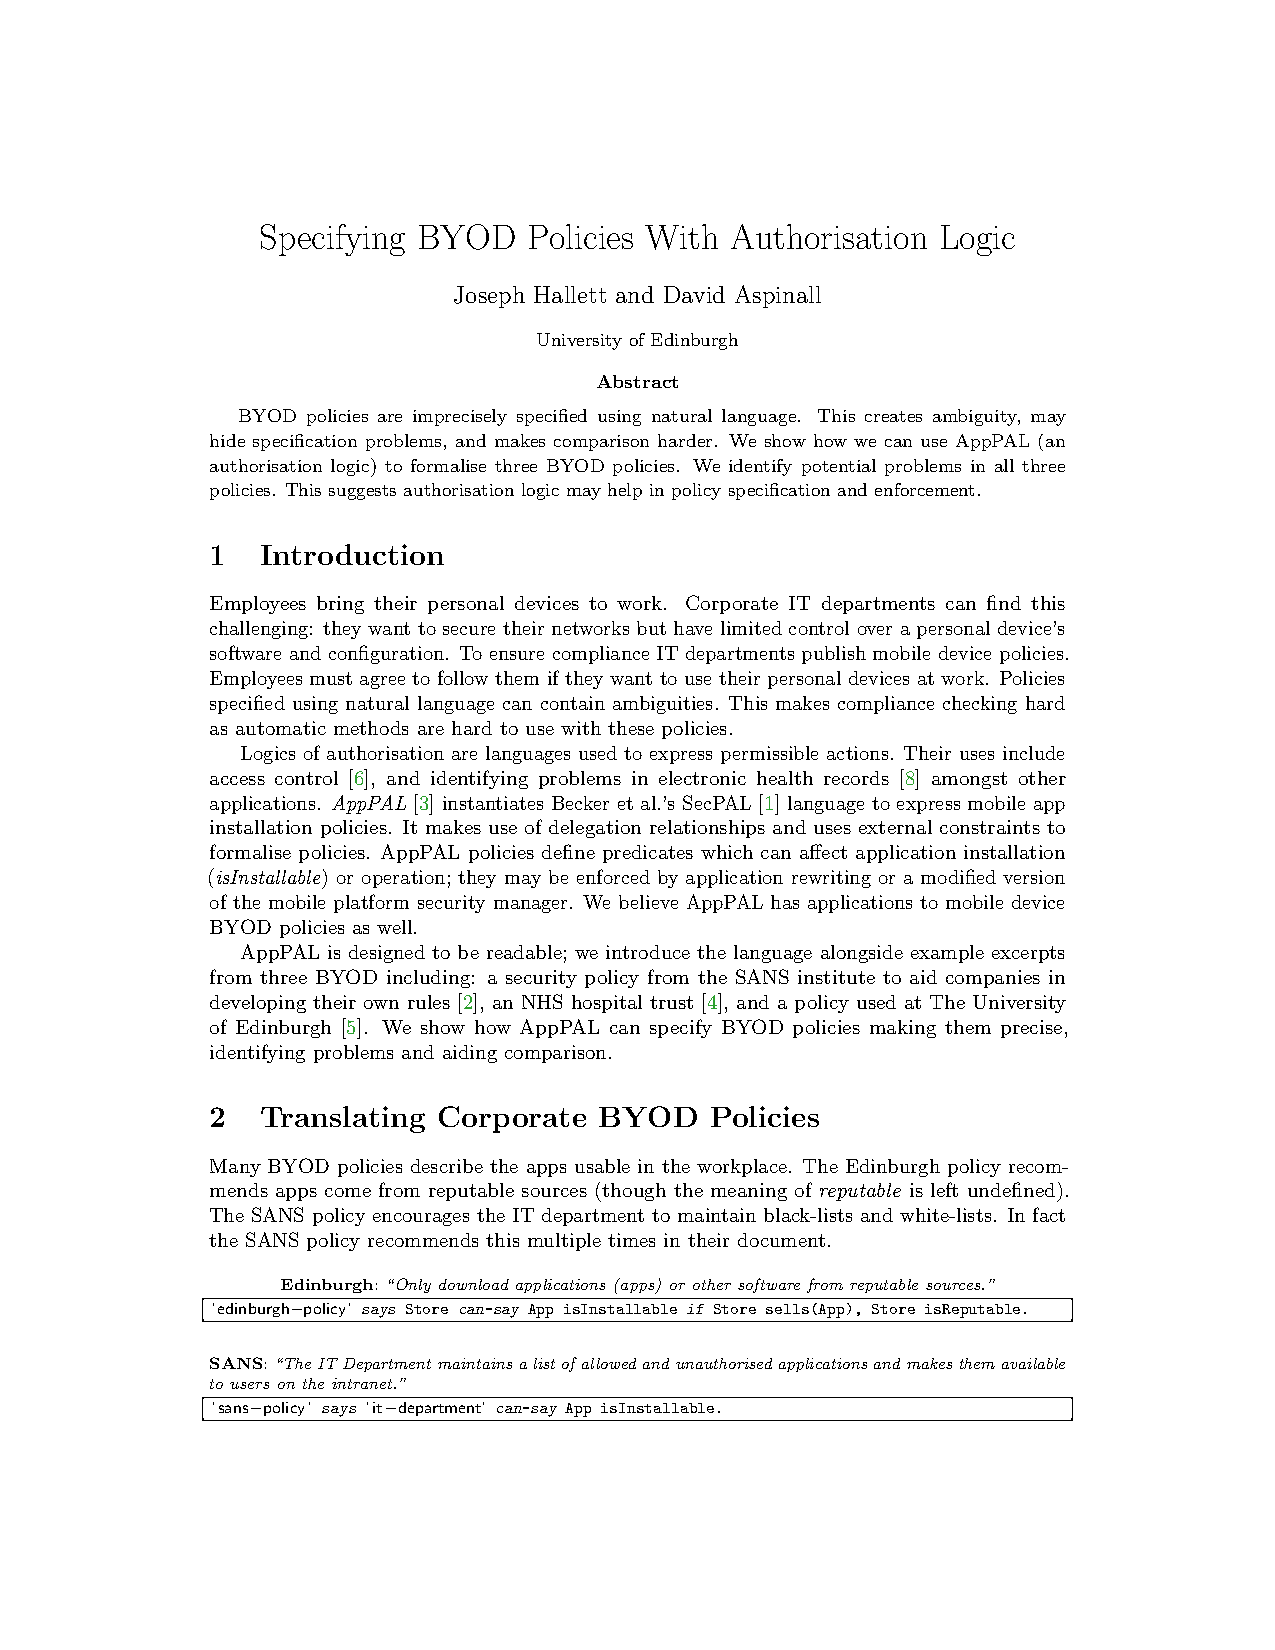
\includepdf[pages=-]{ifm-ds.pdf}



\end{document}
